\section{Introduction}
\label{sec:intro}

Monochrome imaging is important for not only artistic issues 
but also practical applications. 
Despite limited by a less accurate representation of optical
record on sensors, it is expected to retain important and
meaningful visual features and impressions.  
This is especially crucial in vision research, 
as quite a number of techniques in this field work on 
one single color channel in addressing tasks ranging from 
feature extraction to object recognition. 
In this work, we particularly focus on the study of converting
color images into their grayscale, and restrict our discussions to this intriguing category.

From a mathematical viewpoint, decolorizing a color image into
its grayscale counterpart is not a well-posed problem. 
While it is easy to accomplish the task, it is also hard to 
come up with a general and effective solution. 
Among the various approaches, \eg, \cite{Gooch:2005:CSC,Lau:2011:CBC,Ancuti:2011:ESG},
those that can reasonably preserve meaningful visual cues such as edge,
saliency and objectness are deemed to be most useful for computer vision.
While such a goal is explicit, the unavoidable information loss due to 
an underlying projection into the 1-D space of grayscale values has 
preventing the majority of existing techniques from satisfactorily 
performing decolorization. 
The main goal of our research is to propose a new and efficient 
decoloration framework by learning an image-dependent dictionary 
adapted to best characterize color as well as important/salient feature distributions,
and to implicity induce a discriminative feature space of 
higher dimensions to more appropriately account their subtleties.

\begin{figure}[t] 
\begin{center} 
\begin{tabular}{ccc}		
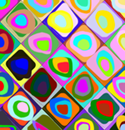
\includegraphics[width=0.25\linewidth]{fig/isoluminance.png} &

\includegraphics[width=0.25\linewidth]{fig/isoluminance-sparse_dr.png} & 

\includegraphics[width=0.25\linewidth]{fig/isoluminance-rgb2gray.png} \\

\includegraphics[width=0.25\linewidth]{fig/rubin_vase.png} & 

\includegraphics[width=0.25\linewidth]{fig/rubin_vase-sparse_dr.png} &

\includegraphics[width=0.25\linewidth]{fig/rubin_vase-rgb2gray.png} \\
(a) Color images & (b) Our results & (c) rgb2gray
\end{tabular} 	
\end{center}
\caption{Visual cues such as edge and objectness may vanish if 
a decolorization method cannot handle isoluminance. 
(The results of rgb2gray are obtained using Matlab.)}
\label{fig:intro}
\end{figure}

In Figure~\ref{fig:intro}, we illustrate examples of losing important information after
performing decolorization. 
There the two color images both contain strong visual cues related to edge,
objectness, and saliency. 
However, using the standard rgb2gray procedure provided in Matlab,
these meaningful features either diminish partially or disappear completely,
as shown in the rightmost column. 
The phenomenon is caused by that the chromatic features
of isoluminance cannot be retained by rgb2gray. 
While this may seem to be inevitable for any legitimate linear projection
to the grayscale, we argue that by transforming to a proper feature space,
the meaningful chromatic and the luminance structures can be better revealed.
In addition, the chance of failing to distinguish different chromatic 
cues of isoluminance would also decrease, 
as the resulting projection is derived based on a new representation designed 
to distinguish the image contents.
